\documentclass[10pt,a4paper]{article}
\usepackage[margin=1.65cm]{geometry}
\usepackage[T1]{fontenc}
\usepackage{lmodern}
\usepackage{microtype}
\usepackage{booktabs}
\usepackage{tabularx}
\usepackage{array}
\usepackage{graphicx}
\usepackage{xcolor}
\usepackage{float}
\usepackage{amsmath}
\usepackage{hyperref}
\usepackage{pgfplots}
\usepackage{tikz}
\pgfplotsset{compat=1.18}
\hypersetup{colorlinks=true,urlcolor=blue!60!black,linkcolor=blue!60!black,citecolor=blue!60!black}
\setlength{\parindent}{0pt}
\setlength{\parskip}{4pt}
\renewcommand{\arraystretch}{1.12}
\newcolumntype{Y}{>{\raggedright\arraybackslash}X}

\begin{document}

\begin{center}
{\LARGE\bfseries MIT 805: Big Data Semester Project}\par
\vspace{2mm}
{\Large Part 2 -- PySpark, MapReduce and Visualisation}\par
\vspace{2mm}
{\large Amazon Reviews 2023: Clothing, Shoes and Jewelry}\par
\vspace{3mm}
\textbf{Group 6:} u26842328 RY Muthadzwi -- u16153970 M Ndlovu
\end{center}

\section{Processing Objective and Analytical Question}

This analysis asks: \emph{Which sufficiently reviewed parent products show the greatest customer-experience risk when review volume, low-rating prevalence, helpful negative feedback, and recent rating change are considered together?} The question converts millions of review events into a transparent product-level prioritisation tool. It is deliberately narrower than general sentiment analysis: the objective is to identify product groups that merit investigation, not to claim that a high score proves a defect.

Five objectives guide the processing: (1) transform raw reviews into valid typed features; (2) demonstrate mapping, shuffle and reduction on the full processing dataset; (3) calculate product-level volume, rating, negative-review and helpfulness measures; (4) compare historical and recent product ratings; and (5) rank stable, sufficiently observed products while retaining the score components for auditability. Products require at least 50 reviews. Part 1 found a 99th percentile of 48 reviews per product, so this rule focuses the analysis on unusually well-observed products and limits instability from very small groups.

\subsection{Dataset scale and subset justification}

The public category file contains 27,810,080,533 bytes (27.810 GB; 25.900 GiB), meeting the 25--40 GB raw-data requirement. The complete downloaded working file has the same size because no filtering was applied. A line-safe prefix containing 3,221,225,482 bytes (3.221 GB; 3.000 GiB) and 7,231,543 complete JSONL records was processed with PySpark 4.0.0. Copying complete lines avoids a corrupt final JSON record. The subset is large enough to demonstrate substantive distributed processing in Colab, but is a sequential prefix and may not reproduce the full file's temporal or product composition.

\begin{table}[H]
\centering\small
\caption{Measured data scale used in Part 2.}
\begin{tabularx}{\textwidth}{@{}lYY@{}}\toprule
Stage & Measured size & Role \\\midrule
Raw & 27,810,080,533 bytes (27.810 GB) & Original public category file \\
Working & 27,810,080,533 bytes (27.810 GB) & Complete downloaded JSONL file \\
Processing & 3,221,225,482 bytes (3.221 GB) & 7,231,543 records processed by Spark \\\bottomrule
\end{tabularx}
\end{table}

\newpage
\section{Mapping and Transformation}

Spark reads the processing JSONL file directly. The analysis selects the parent product, user, rating, helpful-vote, verified-purchase, timestamp and review-text fields. Ratings are cast to double precision, helpful votes and timestamps to long integers, and millisecond timestamps are converted to Spark timestamps. Records without a parent product or with ratings outside 1--5 are excluded.

Each remaining review is mapped to features required by the analytical question:
\begin{itemize}
\item \texttt{is\_negative}=1 for ratings of one or two stars, and \texttt{is\_positive}=1 for four or five stars;
\item \texttt{verified\_flag} converts the Boolean verified-purchase value to an aggregation-ready integer;
\item \texttt{negative\_helpful} retains helpful votes only for negative reviews;
\item \texttt{log1p\_helpful} limits the leverage of the highly right-skewed vote count without discarding popular reviews;
\item \texttt{review\_year} and \texttt{period} distinguish historical reviews (up to 2020) from recent reviews (2021--2023).
\end{itemize}

The transformed DataFrame is repartitioned into 64 partitions by \texttt{parent\_asin} and cached because several downstream aggregations reuse it. These are lazy transformations: Spark records their lineage but does not execute the complete DAG until an action such as \texttt{count()}, \texttt{show()} or \texttt{write()} is requested. All substantive transformations operate on the distributed Spark DataFrame; Pandas receives only bounded aggregate tables for plotting.

\subsection{Explicit MapReduce validation}

An independent RDD pipeline makes the MapReduce semantics explicit. The map step emits
\[
(\texttt{parent\_asin},(1,r,n,h,v)),
\]
where $r$ is the rating, $n$ the negative indicator, $h$ helpful votes attached to negative reviews, and $v$ the verified indicator. \texttt{reduceByKey} combines tuples using associative element-wise addition. It produced 1,836,721 product keys. The resulting counts and sums were compared with the independently implemented DataFrame aggregation; the mismatch count was zero across review count, rating sum, negative count, negative helpful votes and verified count. This agreement provides an auditable correctness check rather than relying on one implementation alone.

\begin{table}[H]
\centering\small
\caption{Map-stage fields and their analytical purpose.}
\begin{tabularx}{\textwidth}{@{}lY@{}}\toprule
Mapped field & Purpose \\\midrule
\texttt{parent\_asin} & Stable key used to bring reviews for the same parent product together. \\
\texttt{rating}, \texttt{is\_negative} & Product mean rating and prevalence of one/two-star feedback. \\
\texttt{negative\_helpful} & Strength of customer endorsement for negative feedback. \\
\texttt{verified\_flag} & Descriptive context for the share of verified reviews. \\
\texttt{period} & Historical-versus-recent rating comparison. \\\bottomrule
\end{tabularx}
\end{table}

\newpage
\section{Shuffle, Reduction and Spark Execution}

\texttt{groupBy(parent\_asin)} creates a wide dependency. Reviews for the same product may begin in different partitions, so Spark hashes the key and moves intermediate records across partitions. The physical plan records this data movement as an \texttt{Exchange}. Spark performs partial \texttt{HashAggregate} operations before the exchange where possible, reducing shuffle volume, then performs final aggregation after related keys are co-located.

For every product, the reduction calculates review count, mean rating, negative count and share, positive count, negative helpful-vote total, verified share, mean log-helpfulness, first year and last year. A second grouped aggregation pivots the two periods and calculates historical and recent means. A key-based left join connects these compact product tables. Products with at least 50 reviews are retained, leaving 17,765 eligible groups.

The interpretable composite score is
\[
R = p_-\log(1+n)\,[1+\log(1+h_-)]\,[1+\max(-\Delta,0)],
\]
where $p_-$ is negative-review share, $n$ review count, $h_-$ helpful votes on negative reviews, and $\Delta$ is recent minus historical mean rating. The logarithms prevent extremely large counts from overwhelming the other components. A decline increases risk; an increase does not reduce the base risk below that implied by negative share, evidence volume and helpfulness.

\subsection{Spark DAG compared with Hadoop MapReduce}

The formatted physical plan contains scans, filters and projections (narrow mapping transformations), \texttt{Exchange} nodes (shuffle boundaries), partial and final \texttt{HashAggregate} stages, a pivot and a sort-merge join. Spark represents this work as a directed acyclic graph and pipelines compatible narrow operations into the same stage. Wide dependencies create stage boundaries and tasks operate on partitions. Adaptive query execution can revise the physical plan using runtime statistics, while caching allows the 7.23-million-row transformed DataFrame to be reused.

Traditional Hadoop MapReduce instead enforces a comparatively rigid Map $\rightarrow$ Shuffle $\rightarrow$ Reduce sequence for each job and typically materialises intermediate output to disk between jobs. Spark can compose multiple transformations and aggregations in one DAG, retain intermediates in memory or memory-and-disk storage, and optimise the complete plan before execution. The explicit RDD operation demonstrates the shared paradigm, while the DataFrame plan demonstrates Spark's modern optimisation.

\begin{table}[H]
\centering\small
\caption{Execution evidence from the verified Colab run.}
\begin{tabularx}{\textwidth}{@{}lY@{}}\toprule
Evidence & Verified value \\\midrule
Spark version and partitioning & PySpark 4.0.0; 64 shuffle and cached-data partitions \\
Processing scale & 7,231,543 valid records \\
RDD reduction output & 1,836,721 parent-product keys \\
Eligible product groups & 17,765 groups with at least 50 reviews \\
Independent validation & 0 RDD/DataFrame aggregation mismatches \\
Plan evidence & \texttt{Exchange}, partial/final \texttt{HashAggregate}, pivot and sort-merge join \\\bottomrule
\end{tabularx}
\end{table}

\newpage
\section{Results and Technical Interpretation}

Eligible products averaged 149.53 reviews and 4.287 stars. Their mean negative-review share was 11.14\%, while the median composite risk score was 1.616. Among 16,535 products with observations in both periods, recent mean rating was on average 0.118 stars below the historical mean. This aggregate decline is descriptive; it does not establish a platform-wide causal trend.

Product \texttt{B019VM3CPW} ranked first with a score of 28.18. It combined 408 reviews, a 26.23\% negative share, 222 helpful votes on negative reviews and a decline from 3.789 historical stars to 2.000 recent stars. Product \texttt{B074TWL5HV} ranked second (26.98) because its much larger evidence base of 2,329 reviews, 37.87\% negative share and 452 helpful negative votes outweighed its smaller 0.291-star decline. The ranking therefore answers the central question by exposing products where several risk signals coincide rather than sorting on mean rating alone.

\begin{table}[H]
\centering\scriptsize
\caption{Ten highest-ranked product-risk signals.}
\begin{tabular}{@{}rlrrrrr@{}}\toprule
Rank & Parent ASIN & Reviews & Mean & Neg. share & Change & Score \\\midrule
1 & B019VM3CPW & 408 & 3.784 & 0.262 & -1.789 & 28.180 \\
2 & B074TWL5HV & 2329 & 3.221 & 0.379 & -0.291 & 26.980 \\
3 & B073D254G5 & 1163 & 3.356 & 0.360 & -0.526 & 23.427 \\
4 & B07KCN4G6T & 5844 & 3.691 & 0.266 & -0.331 & 22.590 \\
5 & B0BS66M37H & 373 & 3.375 & 0.335 & -0.565 & 21.542 \\
6 & B07V33GN1Q & 726 & 3.408 & 0.332 & -0.542 & 20.966 \\
7 & B075B41Y9Z & 1451 & 3.521 & 0.290 & -0.502 & 20.326 \\
8 & B0BN9DY5FV & 4628 & 3.790 & 0.234 & -0.520 & 19.934 \\
9 & B075ZTS57G & 89 & 2.551 & 0.584 & -0.777 & 19.888 \\
10 & B000M85KOQ & 51 & 2.843 & 0.471 & -1.880 & 19.488 \\\bottomrule
\end{tabular}
\end{table}

\begin{figure}[H]
\centering
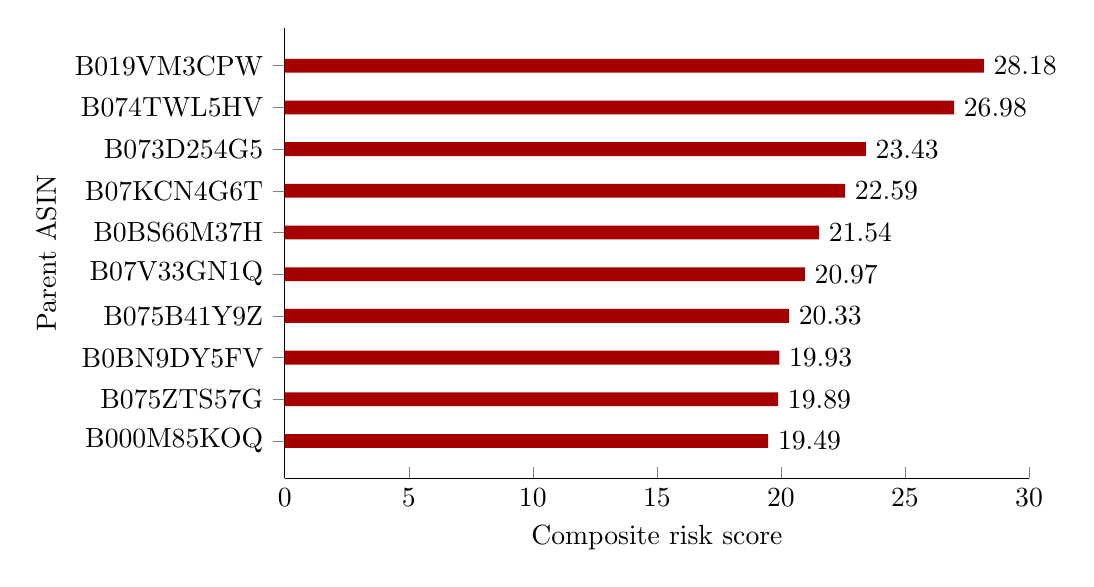
\begin{tikzpicture}
\begin{axis}[
width=.91\textwidth,height=7.3cm,
xbar,xmin=0,xmax=30,
symbolic y coords={B000M85KOQ,B075ZTS57G,B0BN9DY5FV,B075B41Y9Z,B07V33GN1Q,B0BS66M37H,B07KCN4G6T,B073D254G5,B074TWL5HV,B019VM3CPW},
ytick=data,xlabel={Composite risk score},ylabel={Parent ASIN},nodes near coords,
nodes near coords align={horizontal},bar width=5pt,axis x line*=bottom,axis y line*=left,
]
\addplot[fill=red!65!black,draw=none] coordinates {(19.488,B000M85KOQ)(19.888,B075ZTS57G)(19.934,B0BN9DY5FV)(20.326,B075B41Y9Z)(20.966,B07V33GN1Q)(21.542,B0BS66M37H)(22.590,B07KCN4G6T)(23.427,B073D254G5)(26.980,B074TWL5HV)(28.180,B019VM3CPW)};
\end{axis}
\end{tikzpicture}
\caption{The ten highest composite product-risk signals.}
\end{figure}

\newpage
\section{Visualisation and Pattern Interpretation}

Three charts were generated from bounded Spark aggregates. The first ranks high-priority products and makes the score concentration immediately visible. The second plots review count on a logarithmic axis against mean rating for the 5,000 most-reviewed eligible products, with colour representing negative-review share. This prevents a few extremely high-volume products from compressing the remaining points and reveals the expected inverse relationship between mean rating and negative share without implying causation. The third plots recent-minus-historical rating change for 5,000 high-volume products with valid values in both periods. Its zero reference line distinguishes improvement from deterioration.

The rating-band reduction adds an interpretable operational summary: 22 eligible products were below 3.0 stars, 239 were between 3.0 and 3.49, 2,422 were between 3.5 and 3.99, and 15,082 were at least 4.0. The predominance of products above four stars is consistent with the positive rating distribution found in Part 1. Nevertheless, the ranking identifies important exceptions whose evidence volume and negative helpful feedback justify closer inspection.

\begin{figure}[H]
\centering
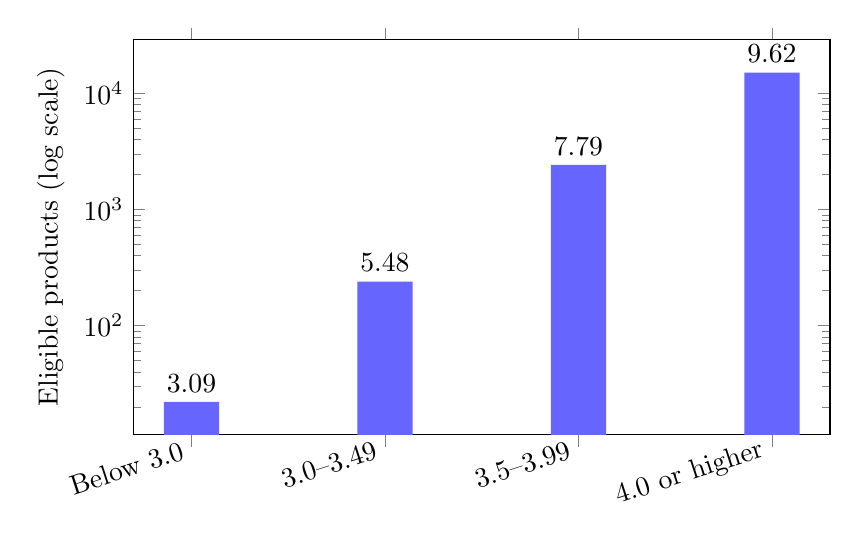
\begin{tikzpicture}
\begin{axis}[
width=.86\textwidth,height=6.6cm,
ybar,bar width=20pt,ymin=0,ymode=log,
symbolic x coords={Below 3.0,3.0--3.49,3.5--3.99,4.0 or higher},xtick=data,
xticklabel style={rotate=18,anchor=east},ylabel={Eligible products (log scale)},
nodes near coords,nodes near coords align={vertical}
]
\addplot[fill=blue!60,draw=none] coordinates {(Below 3.0,22)(3.0--3.49,239)(3.5--3.99,2422)(4.0 or higher,15082)};
\end{axis}
\end{tikzpicture}
\caption{Eligible products by mean-rating band. A log scale preserves visibility of the smaller low-rating groups.}
\end{figure}

\begin{table}[H]
\centering\small
\caption{Distribution summary for eligible products.}
\begin{tabular}{@{}lrrrrrr@{}}\toprule
Statistic & Reviews & Mean rating & Negative share & Neg. helpful & Rating change & Risk score \\\midrule
Mean & 149.53 & 4.287 & 0.111 & 22.41 & -0.118 & 2.194 \\
Median & 87 & 4.322 & 0.100 & 7 & -0.093 & 1.616 \\
75th pct. & 144 & 4.500 & 0.145 & 19 & 0.120 & 2.955 \\
Maximum & 37409 & 4.968 & 0.623 & 3065 & 3.523 & 28.180 \\\bottomrule
\end{tabular}
\end{table}

\newpage
\section{Business and Societal Value}

Retail quality teams can use the ranking as a triage mechanism. High-volume products with unusually high negative share, strongly endorsed negative reviews and recent deterioration can be reviewed before lower-evidence cases. Manufacturers can compare recurring complaints with return, warranty and defect records; merchandising teams can consider whether listing descriptions, variants or sizing guidance create avoidable dissatisfaction; and platform teams can monitor whether recent changes coincide with seller, fulfilment or product-version changes. The score's decomposed components make escalation decisions explainable.

The potential societal value is improved transparency and fewer repeated negative customer experiences. Earlier investigation may identify misleading descriptions, unreliable sizing, durability concerns or safety-related complaints. However, automated removal, seller penalties or safety claims must never be based on this score alone. Human review of the underlying text and relevant operational records is required.

\section{Limitations and Safeguards}

\begin{enumerate}
\item \textbf{Selection bias:} reviews are voluntary and do not represent every purchaser. Very satisfied or dissatisfied customers may be over-represented.
\item \textbf{Subset coverage:} the 3 GiB sequential prefix is computationally practical but may differ from the complete 27.810 GB file in time and product mix.
\item \textbf{Causality:} associations between rating, volume, helpfulness and time do not show that a product caused an outcome or that a particular change caused a decline.
\item \textbf{Product identity:} parent ASINs may combine variants or reflect listing merges; repeated observations are not necessarily independent.
\item \textbf{Platform effects:} incentives, moderation, ranking, coordinated reviews or manipulation can affect both ratings and helpful votes.
\item \textbf{Temporal comparability:} 2023 is partial, and some high-ranked products have few recent observations. Period means should be inspected together with counts before intervention.
\item \textbf{Composite-score sensitivity:} the formula is an interpretable prioritisation rule, not a validated probability of product failure. Alternative weights or thresholds can change rankings.
\end{enumerate}

Operational use should therefore retain component measures, require minimum recent-period evidence, inspect review text and product metadata, test threshold sensitivity, and document any decisions arising from the ranking. Pseudonymous identifiers must not be used for re-identification.

\section{Reproducibility}

The repository contains the PySpark notebook, dependency list, measured evidence, ranked output and reproduction instructions: \url{https://github.com/Rabelani-byte/MIT805-Big-Data-Project}. The shared executed Colab notebook is at \url{https://colab.research.google.com/drive/1RVfabw78yQw_yN5GHJmJzYkiTVJwuTCb}. Raw and processing data are intentionally excluded; the README documents the public source and line-safe recreation process. Commits are attributable to group contributors.

\newpage
\section{Conclusion}

The verified PySpark pipeline transformed 7,231,543 reviews, grouped them into 1,836,721 product keys and identified 17,765 sufficiently reviewed products. Explicit RDD MapReduce and the independent DataFrame reduction agreed with zero mismatches. The Spark plan demonstrates mapping, exchange-driven shuffle, partial and final aggregation, pivoting and joining within a DAG-based execution model. Results identify a concentrated set of products where negative prevalence, evidence volume, helpful negative feedback and recent deterioration coincide. The analysis therefore answers the central question while remaining transparent about uncertainty: the score directs investigation, not automatic judgement.

\section*{References}
\small
\begin{enumerate}
\item J. Hou et al., ``Bridging Language and Items for Retrieval and Recommendation,'' 2024. \url{https://arxiv.org/abs/2403.03952}.
\item McAuley Lab, ``Amazon Reviews 2023,'' Hugging Face dataset repository. \url{https://huggingface.co/datasets/McAuley-Lab/Amazon-Reviews-2023}.
\item Apache Software Foundation, ``Spark Programming Guide'' and ``Spark SQL Performance Tuning.'' \url{https://spark.apache.org/docs/latest/}.
\item MIT 805, ``Big Data Semester Project (2026): Large-Scale Data Analysis and Distributed Processing with PySpark,'' assignment brief.
\end{enumerate}

\section*{Appendix: Video and Evidence Checklist}
The demonstration should show the measured sizes, transformed schema, RDD map and \texttt{reduceByKey}, DataFrame grouping and risk calculation, zero-mismatch validation, \texttt{Exchange}/\texttt{HashAggregate} plan evidence, the three charts, stakeholder interpretation, limitations and GitHub reproduction instructions. The notebook exports \texttt{part2\_evidence.json}, \texttt{part2\_top\_risk\_products.csv}, rating bands, the executed plan and all three figures.

\end{document}
